\todo{PAREI A REVISAO AQUI.}

The goal of the Server Side Application is to process user defined requests, and to construct a solution to them. There are two steps to produce a response to a request: data collection, and optimization. Both of these steps are managed by the SSA, respectively in the Data Management System (DMS) and in the Optimization System (OS). The data collection procedure will be explained with more detail in subsection \ref{sec:dms_implementation}, while the optimization procedure was described in chapter \ref{chap:os}.

The Server Side Application is built using Python and a Python framework denoted Django, which facilitates the construction of servers and APIs. Django enables the creation of routes for the application, and each of these is connected to a particular set of instructions. It is also possible to define a pattern each route, enabling the setting of user selected input. \todo{shit paragraph}

Upon receiving a request, its Uniform Resource Identifier (URI) is used to identify a particular resource, and the set of user selected input. This data is used as input to a python class called \textit{Resource}. Upon creating the Resource object, the user defined request is validated. In case there is an error in the data, for example a past date, or an invalid airport/city, the proccess does not continue, and Django responds with an error. On the other hand, if the validation is succesfull, the Resource object creates a second class object, called \textit{Request} object. There are 3 types of request objects: the \textit{single}, \textit{round} and \textit{multicity} trip. These objects are not to be confused with the respective single/round flight. While a flight corresponds to a single instance connecting two locations in a particular date, a single/round flight may have an extended start period, in which case there are several flights which may constitute a solution to a user request.

Every Request class has a particular set of functions which are executed each time the class is instantiated. This set of instructions are called the \textit{main} cycle of each request object, and correspond to the:

\begin{enumerate}[noitemsep,topsep=0pt,parsep=0pt,partopsep=0pt]
  \item creation of a list of necessary flights;
  \item acquisition of the necessary flight data;
  \item construction of the weight matrix according to the objective function;
  \item execution of the optimization algorithms;
  \item construction of the solution;
\end{enumerate}

From the above defined main cycle, steps i), iii) and v) are done internally, by each of the class object, while steps ii) and iv) are managed by the Data Management and Optimizaion system, respectively. Note that the step iv), the execution of optimization algorithms, is not necessary for the single/round trip objects,
because the best solution is unambiguous.

Figure \ref{fig:api_structure} illustrates the structure of the Client Side Application. This application is activated each time a request is received, which activates  the instantiation of a \textit{Resource} object, responsible for the validation of the request. After a successfull validation, the Resource object instantiates a \textit{Request} object, which executes the \textit{main cycle} of the solution construction procedure, by first calling the Data Management System to collect the necessary set of flights, following this with the execution of a series of optimization algorithms, to produce a stream of responses which can be served to respond to the request.

\begin{figure}[htpb]
  \centering
  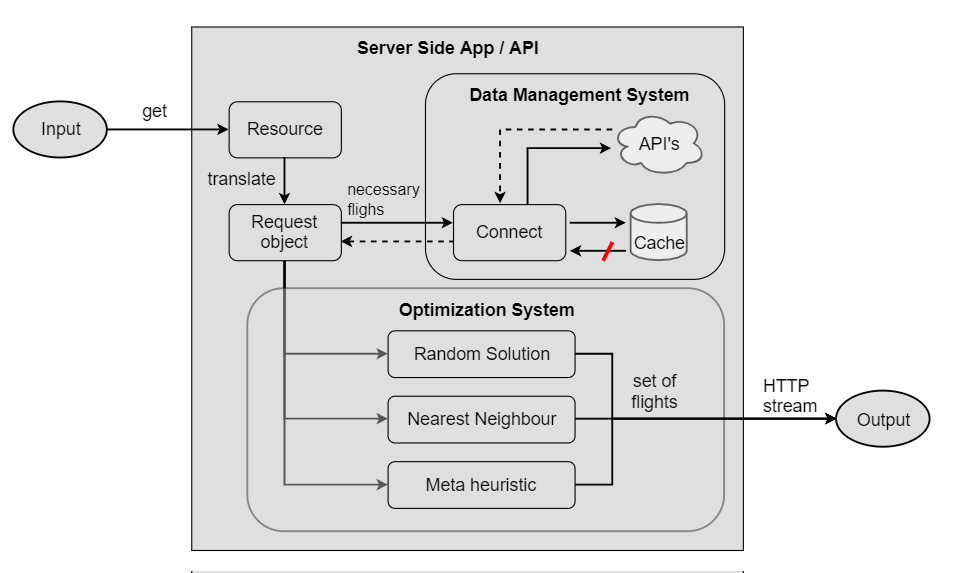
\includegraphics[width=\textwidth]{./Figures/system_implementation/api_structure.png}
  \caption{Structure of the Server Side Application/API.}
  \label{fig:api_structure}  
\end{figure}